\hypertarget{Helpers_8h}{
\section{Helpers.h File Reference}
\label{Helpers_8h}\index{Helpers.h@{Helpers.h}}
}


This graph shows which files directly or indirectly include this file:\nopagebreak
\begin{figure}[H]
\begin{center}
\leavevmode
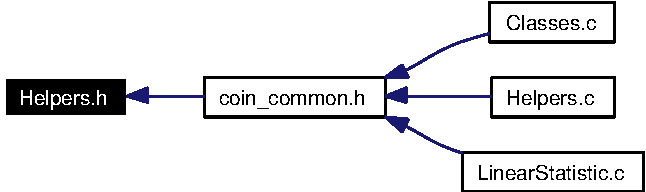
\includegraphics[width=146pt]{Helpers_8h__dep__incl}
\end{center}
\end{figure}
\subsection*{Functions}
\begin{CompactItemize}
\item 
int \hyperlink{Helpers_8h_eeb672a71c45ead28b7b354414f2427a}{nrow} (SEXP x)
\item 
int \hyperlink{Helpers_8h_f1f46cc3e98630497a1ccb21d943fe65}{ncol} (SEXP x)
\end{CompactItemize}


\subsection{Function Documentation}
\hypertarget{Helpers_8h_f1f46cc3e98630497a1ccb21d943fe65}{
\index{Helpers.h@{Helpers.h}!ncol@{ncol}}
\index{ncol@{ncol}!Helpers.h@{Helpers.h}}
\subsubsection{\setlength{\rightskip}{0pt plus 5cm}int ncol (SEXP {\em x})}}
\label{Helpers_8h_f1f46cc3e98630497a1ccb21d943fe65}




Definition at line 22 of file Helpers.c.\hypertarget{Helpers_8h_eeb672a71c45ead28b7b354414f2427a}{
\index{Helpers.h@{Helpers.h}!nrow@{nrow}}
\index{nrow@{nrow}!Helpers.h@{Helpers.h}}
\subsubsection{\setlength{\rightskip}{0pt plus 5cm}int nrow (SEXP {\em x})}}
\label{Helpers_8h_eeb672a71c45ead28b7b354414f2427a}




Definition at line 11 of file Helpers.c.